\documentclass[10pt,twocolumn,letterpaper]{article}

\usepackage{cvpr}
\usepackage{times}
\usepackage{epsfig}
\usepackage{graphicx}
\usepackage{amsmath}
\usepackage{amssymb}
\usepackage{subfigure}

\newcommand{\myfrac}[2]{\textstyle\frac{#1}{#2}\displaystyle}

\long\def\symbolfootnote[#1]#2{\begingroup%
\def\thefootnote{\fnsymbol{footnote}}\footnote[#1]{#2}\endgroup} 

\newcommand{\TODO}{\textcolor{red}{TO DO:~}}
\newcommand{\KEVIN}{\textcolor{blue}{Kevin comment:~}}
\newcommand{\ALEX}{\textcolor{blue}{Alex comment:~}}
\newcommand{\JOHN}{\textcolor{blue}{Alex comment:~}}

\newcommand{\demi}{\myfrac{1}{2}}


\newcommand{\mysec}[1]{Section~\ref{sec:#1}}
\newcommand{\eq}[1]{Eq.~(\ref{eq:#1})}
\newcommand{\myfig}[1]{Figure~\ref{fig:#1}}
\newcommand{\myeq}[1]{Eq.~(\ref{eq:#1})}

\newcommand{\tr}{\text{tr}}
\newcommand{\vect}[1]{\text{vect}\left(#1\right)}

\newcommand{\diag}{\text{diag}}
\newcommand{\Diag}{\text{Diag}}

\newcommand{\xx}{\times}

\newcommand{\BEQAS}{\begin{eqnarray*}}
\newcommand{\EEQAS}{\end{eqnarray*}}

\newcommand{\BIEQAS}{\begin{IEEEeqnarray*}}
\newcommand{\EIEQAS}{\end{IEEEeqnarray*}}

\newcommand{\BEQA}{\begin{eqnarray}}
\newcommand{\EEQA}{\end{eqnarray}}

\newcommand{\BIEQA}{\begin{IEEEeqnarray}}
\newcommand{\EIEQA}{\end{IEEEeqnarray}}

\newcommand{\idm}{I}

\newcommand{\Simp}{\mathcal {S}}
\def\R{{\rm I}\!{\rm  R}}
\newcommand{\C}{\mathcal {C}}
\newcommand{\LL}{\ell}
\newcommand{\EE}{\mathbb {E}}
\newcommand{\Ecal}{\mathcal {E}}
\newcommand{\I}{\mathbbm {1} }

\newcommand{\mcal}[1]{\mathcal{#1}}
\newcommand{\bb}[1]{\mathbb{#1}}

\newcommand{\Fa}{J_{\alpha}}
\newcommand{\Fwb}{J_{w b}}
\newcommand{\Fapp}{J_{\text{app}}}


\newcommand{\suce}{\preccurlyeq}
\newcommand{\estSuce}{\succcurlyeq}

\newcommand{\logPartNS}{A_0(W,b)}
\newcommand{\logPart}[1]{A_{#1}(W,b)}
\newcommand{\psiPara}{\tau}

\newcommand{\sumL}{\sum_{l=1}^K}
\newcommand{\sumK}{\sum_{k=1}^K}
\newcommand{\sumN}{\sum_{n=1}^N}
\newcommand{\sumM}{\sum_{m=1}^M}
\newcommand{\sumR}{\sum_{r=1}^R}
\newcommand{\sumP}{\sum_{p=1}^P}
\newcommand{\sumKL}{\sum_{k,k'=1}^K}

\newtheorem{theorem}{Theorem}[section]
\newtheorem{proposition}[theorem]{Proposition}

\newcommand{\BITE}{\begin{equation}\left\{ \begin{array}{lll}}
\newcommand{\EITE}{\end{array}\right.\end{equation}}

\newcommand{\BITES}{\begin{equation*}\left\{ \begin{array}{lll}}
\newcommand{\EITES}{\end{array}\right.\end{equation*}}








\newcommand{\eat}[1]{}
\newcommand{\Jon}[1]{\textcolor{blue}{\textbf{Jon comment}:~#1}}
\newcommand{\Kevin}[1]{\textcolor{red}{\textbf{Kevin comment}:~#1}}

% Include other packages here, before hyperref.

% If you comment hyperref and then uncomment it, you should delete
% egpaper.aux before re-running latex.  (Or just hit 'q' on the first latex
% run, let it finish, and you should be clear).
\usepackage[pagebackref=true,breaklinks=true,letterpaper=true,colorlinks,bookmarks=false]{hyperref}

% \cvprfinalcopy % *** Uncomment this line for the final submission

\def\cvprPaperID{304} % *** Enter the CVPR Paper ID here
\def\httilde{\mbox{\tt\raisebox{-.5ex}{\symbol{126}}}}

% Pages are numbered in submission mode, and unnumbered in camera-ready
\ifcvprfinal\pagestyle{empty}\fi
\begin{document}


%%%%%%%%% TITLE
%\title{Attend to the player: Player attention for event detection}
%\title{Event detection in videos with attention based key person identifcation}
\title{Detecting events and key actors in multi-person videos}

\author{First Author\\
Institution1\\
Institution1 address\\
{\tt\small firstauthor@i1.org}
% For a paper whose authors are all at the same institution,
% omit the following lines up until the closing ``}''.
% Additional authors and addresses can be added with ``\and'',
% just like the second author.
% To save space, use either the email address or home page, not both
\and
Second Author\\
Institution2\\
First line of institution2 address\\
{\tt\small secondauthor@i2.org}
}

\maketitle
%\thispagestyle{empty}

\begin{abstract}
Multi-person event recognition is a challenging task,
often with many people active in the scene but only a small subset contributing
to an actual event. In this paper, we propose a model which learns to detect events
in such videos while automatically ``attending'' to the people responsible
for the events, without being explicitly told who or where those people are
during training and testing.  In
particular, we detect people in videos and learn time-varying attention
weights to combine their features at each time-instant.  The attended features
are then classified with a Long Short-Term Memory (LSTM) model. 
Since most video datasets with multiple people are restricted to a small
number of videos, we also collected a new basketball dataset comprising 257 basketball games with
14K event annotations corresponding to 11 event classes.  Our model outperforms
state-of-the-art methods for both event classification  and  detection on this
new dataset. Additionally, we show that the attention mechanism is able to localize the
relevant players.
\end{abstract}



\section{Introduction}
When observing a scene, we posess the inate ability to filter out unwanted
stimuli \cite{Desimone_ARN95} and focus only on a selected subset of objects.
This effect is easily understood in the context of multi-player sports, where
we look at only a few key players (Fig.~\ref{fig:pull_figure}) to understand a
complete event. Motivated by this observation, we present an event detection
method which automatically ``attends" to the most releavant person during
different phases of a multi-player event.

\begin{figure}[ht!]
\begin{center}
\fbox{\rule{0pt}{2in} \rule{.9\linewidth}{0pt}}
\end{center}
   \caption{Pull figure.}
\label{fig:pull_figure}
\end{figure}

Acitivity and event recognition in videos has hugely benefited with the
introduction of many recent large scale datasets \cite{}. However, most of
these dataset focus on activities performed by a single person.  Multi-person
datasets like \cite{} are usually restricted to fewer videos.  Further, to
evaluate event detection, it is desirable to have temporal annotations in long
untrimmed videos. Since the focus of our work is towards multi-person actions,
we propose a new dataset of basketball events with time-stamp annotations for
all occurrences of $11$ different events across $257$ videos each $1.5$ hours
long in length.  This dataset is comparable to the THUMOS \cite{THUMOS}
detection dataset in terms of number of annotations and contains longer videos
catering to a multi-person setting.

In basketball, many players are always present in the court.
However, an interesting event like a ``layup" or ``steal" can be attributed
to just one or two players at the scene. Observing these people at the right
time holds the cue to understanding the entire event. Furhter, identifying
these players responsible for the event is an interesting task in its own right.
Hence, it is natural to develop a model which can ``attend" to these players during
an event.

Recently, Recurrent Neural Network (RNN) models have been successful in
using ``attention" \cite{Bahdnau_arxiv14,Xu_arxiv15,Yao_arxiv15} for aligning
elements from an input sequence to those of an output sequence. In these settings,
the input sequence remains fixed at all times and the model chooses from this
fixed input at each instant. However, the use of such attention based RNNs
poses two challenges in our setting:
1. The set of player detections varies from one frame to the other and
2. The model needs to adapt attention according to the phase of the game as
shown in Fig.~\ref{fig:pull_figure}. This presents interesting choices
for the attention model.

While it is possible to treat player detections across frame to be
disconnected, in practice the detections belong to the same set of plyers. We
could leverage this knowledge by using a player tracker followed by better
player representations. However, this could lead to additional issues due to
erroneous tracking and could possibly lower the effectiveness of attention
itself. On the other hand, it is more lucrative to develop an attention model
without tracking.  This could provide more freedom to switch attention between
detections based on the state of the event. We explore both these choices in
our work and compare their event recognition performance as well as ability to
attend to the right players.

The main contribution of our works is to:
1. present a time-varying attention model for basketball event detection
in the presence and absence of player-tracking, 2. We provide a comprehensive
evaluation of the attention scores generated by our model and show
their interpretability in our setting and 3. We introduce a novel
large-scale basketball event dataset with 14K dense temporal annotations
for long video sequences. We outpuerform state-of-the-art
event recognition methods on the new dataset.




\begin{figure*}[ht!]
  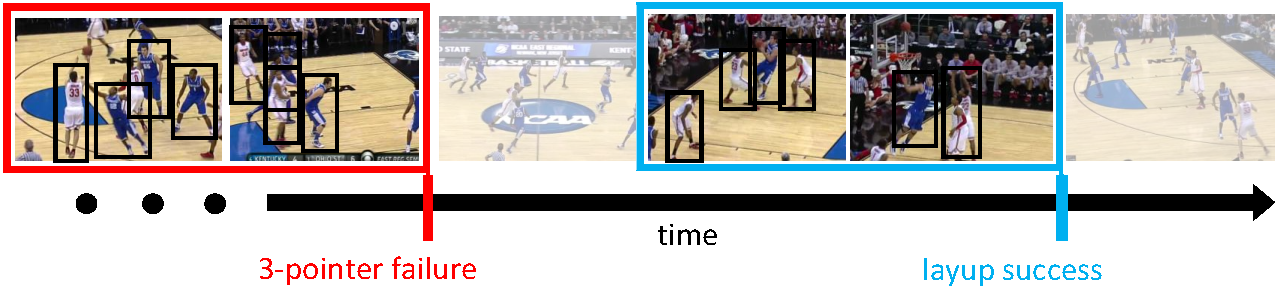
\includegraphics[width=6.5 in]{images/dataset_figure_cropped.pdf}
  \caption{Our dataset contains timestamp annotations for 11 basketball events
    in long untrimmed videos. Additionally, we also provide bounding boxes for player
    detections obtained from a multibox model trained on a subset of training
  video frames.}
\end{figure*}



\section{Related Work}


\noindent \textbf{Action recognition datasets}
Various datasets have been proposed for action recognition,
including KTH \cite{KTH}, HMDB \cite{HMDB}
UCF101 \cite{UCF101}, TRECVID-MED \cite{MED11} and Sports-1M \cite{Karpathy_CVPR14}.
More recently, THUMOS \cite{THUMOS} and ActivityNet \cite{ActivityNet} also provide a detection
setting with temporal annotations for the location of the action in a temporally untrimmed video.
There are also fine-grained datasets
in specific domains such as MPII cooking \cite{Finegrained_cooking} and breakfast \cite{Breakfast}.
However, most of these dataset focus on single-person activities with little
need to recognize the people responsible for the event. On the other
hand, publicly available multi-person activity datasets 
such as \cite{Choi_ICCV09,Ryoo_10} are restricted
to a very small number of videos.  One of the contributions of our work is 
a multi-player basketball dataset with dense temporal event annotations in
long videos, which we discuss in Section~\ref{sec:data}.

\noindent \textbf{Action recognition in videos}
Traditionally, well engineered features have proved quite effective for video
classification and retrieval tasks
\cite{Dalal_ECCV06,Jain_CVPR13,Jiang_ECCV12,Laptev_CVPR08,
Niebels_ECCV10,Oh_MVA14,Oneata_ICCV13,Peng_ECCV14,Sadanand_CVPR12,Wang_BMVC09,Wang_CVPR11}.
The improved dense trajectory (IDT) features \cite{Wang_CVPR11} achieve
competetive results on standard video datasets.  In the last few years,
end-to-end trained deep network models
\cite{Ji_PAMI13,Karpathy_CVPR14,Simonyan_2014,Tran_arxiv14} were shown to be comparable and
at times better than these features for various video tasks.  Other works like
\cite{Xu_2015,Zha_2015,Wang_arxiv15} explore methods for pooling such
features for better performance.

Recent works using Recurrent Neural Networks (RNN) have achieved
state-of-the-art results for both event recognition and caption-generation
tasks \cite{Donahue_arxiv14,Ng_arxiv15,Srivastava_2015,Yao_arxiv15}.
We follow this line of work with addition of attention mechanism
to attend to the event participants.

\noindent \textbf{Muti-person video analysis}
Activigy recognition models for events with well defined group structures such
as parades have been presented in
\cite{Vaswani_CVPR03,Intille_CVIU01,Moore_AAAI02,Khan_ACM05}.  They utilize the
structured layout of participants to identify group events. More
recently, \cite{Lan_PAMI12,Choi_ICCV09,Khodabandeh_arxiv15} use context as a
cue for recognizing interaction based group activities.  While the models
multi-person events, these methods are restricted to smaller
datasets such as UT-Interaction\cite{Ryoo_10}, Collective activity
\cite{Choi_ICCV09} and Nursing home\cite{Lan_PAMI12}.

\noindent \textbf{Attention models}
Itti et al. \cite{Itti_PAMI98} explored the idea of saliency based attention in
images, with other works like \cite{Shapovalova_NIPS13} using eye-gaze data as
a means for learning attention.
Other approaches such as Gkioxari et al. \cite{Gkioxari_arxiv14} and Raptis et al. \cite{Raptis_CVPR12}
automatically localize a spatio-temporal tube in the video corresponding to the action.
Another similar work\cite{Gkioxari_ICCV15} localize boxes in static images
for action recognition.

Recently, \cite{Bahdnau_arxiv14} showed that
attention based RNN models can effectively align input words in a sentence to
output words for machine translation.  Following this work, attention was used
for aligning regions in an image to output words for image-captioning
\cite{Xu_arxiv15} and frames in a video with output words for video-captioning
\cite{Yao_arxiv15}.  In all these methods, attention aligns a sequence of input
features with words of an output sentence. However, in our work we use
attention to identify the most releavant person to the overall event during
different phases of the event.  Further, in our setting the attended set of
player detections changes between frames. This leads to interesting
model choices, which we will discuss in Section~\ref{sec:methods}.

\noindent \textbf{Action recognition datasets}
Action recognition in videos has eveolved with the introduction of more
sophisticated datasets starting from smaller KTH \cite{KTH}, HMDB \cite{HMDB}
to larger , UCF101 \cite{UCF101}, TRECVID-MED \cite{MED11} and Sports-1M \cite{Karpathy_CVPR14}
datasets.
More recently, THUMOS \cite{THUMOS} and ActivityNet \cite{ActivityNet} also provide a detection
setting with temporal annotations for actions in untrimmed videos.
There are also fine-grained datasets
in specific domains such as MPII cooking \cite{Finegrained_cooking} and breakfast \cite{Breakfast}.
However, most of these dataset focus on single-person activities with hardly
any need for recognizing the people responsible for the event. On the other
hand, publicly available multi-person activity datasets \cite{Choi_ICCV09,Ryoo_10,VIRAT} are restricted
to a very small number of videos.  One of the contributions of our work is 
a multi-player basketball dataset with dense temporal event annotations in
long videos. We provide more details in the next section.

\noindent \textbf{Person detection and tracking}. There is a very
large literature on person detection and tracking. Here we just
mention a few key papers.
For person detection, we use the CNN-based multibox detector from
\cite{Szegedy13}.
For person tracking, we use the KLT tracker from
\cite{Veenman_PAMI2001}.
There is also work on player identification (e.g., \cite{Lu2013}), but
in this work, we do not attempt to distinguish individual players.



\section{NCAA Basketball Dataset}
We are not only interested in detecting events in long untrimmed videos, but
also automatically identifying the people responsible for the events.

Unfortunately, recent activity detection datasets like THUMOS \cite{THUMOS},
ActivityNet \cite{ActivityNet}, and others such as
\cite{UCF101,Finegrained_cooking} mostly contain videos with a single actor
where every action is performed in a different setting. These are actions from
multiple sports events and/or household chores.  Identying the person
responsible for the action is not an interesing task in these datasets, and is
not critical for recognizing the action itself.

We focus on a multi-person setting where the events can be primarily
differentiated by the action of a small subset of people present in the scene.
Here, attending to the releavant people becomes more crucial and is a valuable
output in itself. A natural choice for such events is a multi-player sport.
With this in mind, we have collected a new large-scale dataset of basketball
events. This dataset will be made publicly available upon publication.

\subsection{Data Collection}
We needed a large collection of publicly available videos to construct the dataset.
Incidentally, complete basketball videos are
publicly available for $296$ NCAA games on
YouTube\footnote{https://www.youtube.com/user/ncaaondemand}.  These games are
played in different venues over different periods of time with a good amount of
diversity in setting and gameplay across the videos. More interestingly, they
are also accompanied by sparse play-by-play text snippets describing the events
at a few key-moments in each game.

We only consider the most recent $257$ games and ignore the older games with
slightly different rules than modern basketball.  As a first step, we clustered the
play-by-play text to identify the most frequent events from all games. We
narrowed the event list to $11$ classes. These included 5 types of shots and
steal, with each shot being further classified as a successful or failed
attempt (Fig.~\ref{fig:data_dist}). We then setup an AMT task, where the
annotators were asked to annotate the ``end-point" of these events if and when
they occur in the videos. Most basketball shots are of fixed duration. Hence,
we treat a 4 second window around the annotated ``end-point" as the total span
of the event.  Refer to supp. material for more details of the AMT task.

The videos were randomly split into $212$ training, $12$ validation and $33$
test videos. This accounted for a total of $11436$ training, $856$ validation
and $2256$ test event annotatoins. Note that the total number of training and
validation event annotations are comparable to the ongoing THUMOS'15 detection
challenge ($XXXX$ trimmed training instances for $20$ classes and $6553$
untrimmed validation instances). The distribution of annotations across all the
different events is visualized in Fig.~\ref{fig:data_dist}, with sample videos
for a few event classes. The annotations cover all occurrences of the
events in each video. The videos are typically $1.5$ hours long.  To the best of our
knowledge, this is the first dataset with dense temporal annotations for
such long video sequences.


\section{Our Method}
\label{sec:methods}

All events in a team sport are performed in the same scene by the same set
of players. The only basis for differentiating these events is the action
performed by a small subset of people at a given time.  For instance, a
``steal" event in basketball is completely defined by the action of the player attempting to
pass the ball and the player stealing from him.  To understand such an event,
it is sufficient to observe only the players participating in the event.

This motivates us to build a model (overview in Fig.~\ref{fig:model})
which can reason about an event by focusing
on specific people during the different phases of the event.
In this section, we describe our unified model for classifying events
and simultaneously identifying the key players.

\begin{figure}[t!]
\begin{center}
    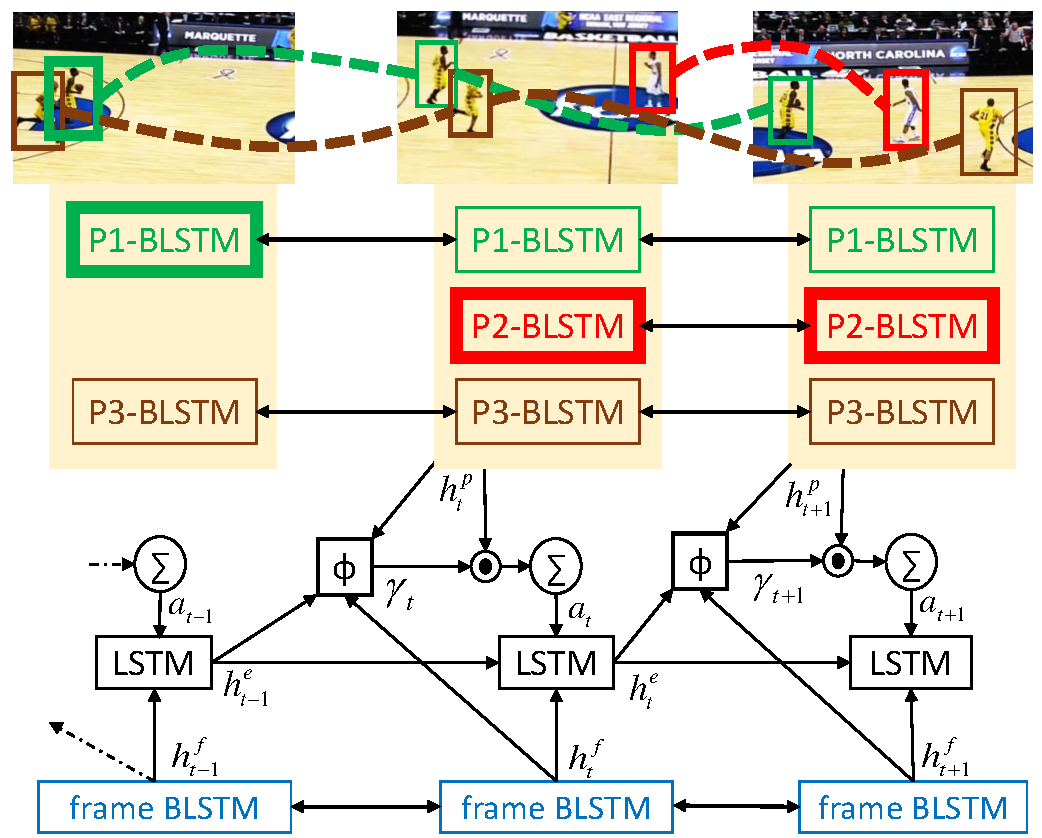
\includegraphics[width=3 in]{images/system_figure_1_cropped_v2.pdf}
\end{center}
   \caption{Our model, where each player track is first processed by the
     corresponding BLSTM network (shown in different colors). The BLSTM
     hidden-states are then used by an attention model to identify the ``key"
     player at each instant.  The thickness of the BLSTM boxes shows the
     attention weights, and the attended person can change with time.  The
     variables in the model are explained in the methods section.  BLSTM stands
     for ``bidirectional long short term memory''. 
     \Jon{add text labels to figure to denote ``player tracks'' and ``event state''}
}
\label{fig:model}
\end{figure}

\subsection{Feature extraction}
\label{sec:feature_extraction}
Each video-frame is represented by a feature vector $f_t$, which is the
activation of the last fully connected layer of the Inception7 network
\cite{Ioffe_arxiv15,Inception7}.  In addition, we compute spatially localized
features for each person in the frame. In particular, we compute a feature
vector $p_{ti}$ which contains both appearance and spatial information for the
$i$'th player bounding box in frame $t$.
Similar to the RCNN object
detector\cite{Girshick_CVPR14}, the appearance features were extracted by feeding the cropped
and resized player region from the frame through the Inception7 network and
spatially pooling the response from a lower layer. The spatial feature
corresponds to a $32\times 32$ spatial histogram, combined with a spatial pyramid, to
indicate the bounding box location at multiple scales.
While we have only used spatial CNN representations in our
work, these features can also be easily extended with flow information as
suggested in \cite{Simonyan_NIPS14}.

\subsection{Event classification}

Given $f_t$ and $p_{ti}$ for each frame $t$ from $1$ to $T$, our goal
is to train the model to classify the clip into one of 11 categories. As a side
effect of the way we construct our model, we will also be able to identify the
key player in each frame.

First we compute a global context feature for each frame, $h_t^f$, derived from
a bidirectional LSTM applied to the frame-level feature as shown 
by the blue boxes in Fig.~\ref{fig:model}.
This is a concatenation of the hidden states from the forward and reverse LSTM
components of a BLSTM and can be compactly represented as:
\[
  h_t^f = \mbox{BLSTM}_{frame}(h_{t-1}^f, h_{t+1}^f, f_t).
\]Please refer to Graves et al. \cite{Graves_2013} or the supp. material
for the full equations.

Next we use  a unidirectional LSTM to represent the state of the
event at time $t$:
\begin{equation}
  \label{eq:event_lstm}
h_t^e = \mbox{LSTM}(h_{t-1}^e, h_t^f, a_t),
\end{equation}
where $a_t$ is a feature vector derived from the players, as we
describe below.
From this, we can predict the class label for the clip using $w_k^T
h_t^e$. We measure the squared-hinge loss as follows:
\begin{equation}
  L =   \frac{1}{2} \sum_{t=1}^T \sum_{k = 1}^K \max (0, 1 - y_k w_k^T h^e_t)^2,
\end{equation} 
where $y_k$ is $1$ if the video belongs to class $k$,
and is $-1$ otherwise, and the weight vector corresponding to
class $k$ is denoted by $w_k$.

\subsection{Attention models}
Unlike past attention models \cite{Bahdnau_arxiv14,Xu_arxiv15,Yao_arxiv15} we need to attend to a different set of
features at each time-step. There are two key issues to address in this
setting.

First, although we have different detections in each frame, they
can be connected across the frames through an object tracking
method. This could lead to better feature representation of the
players.

Second, player attention depends on the state of the event and needs to evolve
with the event.  For instance, during the start of a ``free-throw" it is
important to attend to the player making the shot. However, towards the end of
the event the success or failure of the shot can be judged by observing the
person in possession of the ball.

With these issues in mind, we first present our model which uses player tracks
and learns a BLSTM based representation for each player track. Next, we also
present a simple tracking-free baseline model.

\noindent \textbf{Attention model with tracking.}
We first associate the detections
belonging to the same player into tracks using a standard
tracking method. We use a KLT tracker combined with
bipartite graph matching \cite{munkres1957algorithms} to perform the data association.

The player tracks can now be used to incorporate context
from adjacent frames while computing their representation.
We do this through a separate BLSTM which learns a latent
representation for each player at a given time-step.
The latent representation of player $i$ in frame $t$ is
given by the hidden state
$h_{ti}^p$ of the BLSTM across the player-track:
\[
  h_{ti}^p = \mbox{BLSTM}_{track}(h_{t-1,i}^p, h_{t+1,i}^p, p_{ti}).
\]

At every time-step we want the most relevant player at that
instant to be chosen. We achieve this by computing
$a_t$ as a convex combination of the player representations
at that time-step:
\begin{eqnarray} 
\label{eq:track}
  a_t^{track} & = & \sum_{i=1}^{N_t} \gamma_{ti}^{track} h_{ti}^p, \\ \nonumber
  \gamma_{ti}^{track} & = & \text{softmax} \left(\phi\left(h^f_t, h^p_{ti}, h^e_{t-1}\right); \tau\right),
\end{eqnarray}where $N_t$ is the number of detections in frame $t$, and $\phi()$ is a 
multi layer perceptron, similar to \cite{Bahdnau_arxiv14}. $\tau$ is the softmax temperature parameter.
This attended player representation is input to the
unidirectional event recognition LSTM in Eq.~\ref{eq:event_lstm}.

This model is illustrated in Figure~\ref{fig:model}.
Later, we show that this method achieves better
performance at event classification and detection compared to a
tracking-free model (discussed next). However, it could result in slightly worse ``key player"
identification due to tracking errors.

\noindent \textbf{Attention model without tracking.}
Often, tracking people in a crowded scene can be very difficult due to
occlusions and fast movements. In such settings, it is beneficial to have a
tracking-free model.  As an added benefit, this could allow the model to be
more flexible in switching attention between players as the event progresses.
Motivated by this, we present a model where the detections in each frame are
considered to be independent from other frames. 

We  compute the (no track) attention based player feature as shown below:
\begin{eqnarray} 
\label{eq:notrack}
  a_t^{notrack} & = & \sum_{i=1}^{N_t} \gamma_{ti}^{notrack} p_{ti},
\\ \nonumber
  \gamma_{ti}^{notrack} & = & \text{softmax} \left(\phi\left(h^f_t, p_{ti}, h^e_{t-1}\right); \tau\right),
\end{eqnarray}

Note that this is similar to the tracking based attention equations except for
the direct use of the player detection feature $p_{ti}$ in place of the
BLSTM representation $h_{ti}^p$.


\section{Experimental evaluation}
\label{sec:experiments}

\begin{table*}[ht!]
\begin{center}
\small
 \begin{tabular}{|l|c|c|c|c|c|c|c|c|c|}
  \hline
Event & IDT\cite{Wang_CVPR11} & IDT\cite{Wang_CVPR11} player & C3D \cite{Tran_arxiv14} & MIL\cite{Andrews_NIPS02} &  LRCN \cite{Donahue_arxiv14} &Only player & Avg. player & Our no track & Our track \\ \hline \hline

  3-point succ.    & 0.370 & 0.428 & 0.117 & 0.237 & 0.462   & 0.469 & 0.545 & 0.583 & \textbf{0.600} \\
  3-point fail.    & 0.501 &  0.481& 0.282 & 0.335 & 0.564   & 0.614 & 0.702 & 0.668 & \textbf{0.738} \\
  fr-throw succ. & 0.778 &  0.703& 0.642   & 0.597 & 0.876   & 0.885 & 0.809 & \textbf{0.892} & 0.882 \\
  fr-throw fail. & 0.365 &  0.623& 0.319   & 0.318 & 0.584    & \textbf{0.700} & 0.641 & 0.671 & 0.516 \\
  layup succ.      & 0.283 & 0.300 & 0.195 & 0.257 & 0.463   & 0.416 & 0.472 & 0.489 & \textbf{0.500} \\
  layup fail.      & 0.278 &0.311  & 0.185 & 0.247 & 0.386   & 0.305 & 0.388 & 0.426 & \textbf{0.445} \\
  2-point succ.    & 0.136 &  0.233 & 0.078& 0.224 & 0.257    & 0.228 & 0.255 & 0.281 & \textbf{0.341} \\
  2-point fail.    & 0.303 &  0.285 & 0.254& 0.299 & 0.378   & 0.391 & \textbf{0.473} & 0.442 & 0.471 \\
  sl. dunk succ.  & 0.197 &  0.171 & 0.047 & 0.112 & 0.285   & 0.107 & 0.186 & 0.210 & \textbf{0.291} \\
  sl. dunk fail.  & 0.004 &  0.010 & 0.004 & 0.005 & \textbf{0.027} & 0.006 & 0.010 & 0.006 & 0.004 \\
  steal            & 0.555 &  0.473& 0.303 & 0.843 & 0.876 &  0.843 & \textbf{0.894} & 0.886 & 0.893 \\ \hline \hline
Mean             & 0.343 &  0.365 & 0.221  & 0.316 & 0.469 & 0.452 & 0.489 & 0.505 & \textbf{0.516} \\ \hline
  \end{tabular}
\end{center}
  \caption{Mean average precision for event {\em classification} given
    isolated clips.}
  \label{tab:event_class}
  \label{tab:class_res}
\end{table*}


In this section, we present three sets of experiments on the NCAA basketball
dataset: 1. event classification, 2. event detection and 3. evaluation of
attention

\subsection{Implementation details}

 We used a hidden state dimension of $256$ for all the LSTM and
BLSTM RNNs, an embedding layer with ReLU non-linearity and $256$ dimension for
embedding the player features and frame features before feeding to the RNNs.
We used $32 \times 32$ bins with spatial pyramid pooling for the player appearance
feature.
All the event videos clips were four seconds long and subsampled to 6fps.  The
$\tau$ value was set to $0.25$ for the attention softmax weighting. We used a
batch size of $128$, learning rate of $0.005$ which was reduced by a factor of
$0.1$ every $10000$ iterations with RMSProp\cite{RMSProp}. The models were trained on
a cluster of $20$ GPUs for $100k$ iterations over one day.
The hyperparameters were chosen by cross-validating on the
validation set.

\subsection{Event classification}

In this section, we compare the ability of methods to perform 11-way classification of isolated video clips.
In this setting, we do not use any
additional negatives from other parts of the basketball videos.
We compare our results
against different control settings and baseline models as explained
below:

\begin{itemize}
  \item \emph{IDT\cite{Wang_CVPR11}} We use the publicly available implementation of dense trajectories with
  Fisher encoding.
  
  \item \emph{IDT\cite{Wang_CVPR11} player} We use IDT along with averaged features extracted from the player
  bounding boxes.

  \item \emph{C3D \cite{Tran_arxiv14}} We use the publicly available pre-trained model for feature extraction
  with an SVM classifier.

  \item \emph{LRCN \cite{Donahue_arxiv14}} This is a baseline model where we use a simple BLSTM on frame-level features similar
  to LRCN. The only difference is the use of BLSTM in place of LSTM. We found this to improve
  performance.

  \item \emph{MIL \cite{Andrews_NIPS02}} Since each frame can be seen as a bag of player features, we used the
  classical MIL model. 

  \item \emph{Only player} We only use player features without frame-level
  features.
 
  \item \emph{Avg. player} We combine the player features by simple averaging, without
using  attention.

  \item \emph{Attn. no track} Our attention model without tracks.

  \item \emph{Attn. with track} Our attention model with tracking.
\end{itemize}

The mean average precision (mAP)
are shown in Tab.~\ref{tab:class_res}. We see that the method that
uses both global information and local player information outperforms
only using player information. We also show that combining the player
information using a weighted sum (i.e., an attention model) is better
than uniform averaging, with the tracking based version of attention
slightly better than the track-free version.
Note that the performance is much poorer (for all methods) for classes
such as ``slam dunk fail'' for which we have very little data.


\subsection{Event detection}

In this section, we evaluate the ability of methods to temporally localize events in untrimmed videos.
We use a sliding window approach, where we slide a $4$ second window
through all the basketball videos and try to classify the window into a negative
class or one of the 11 event classes. We use a stride length of $2$ seconds.
We treat all windows which do not overalp more than $1$ sec with any of the $11$ annotated
events as negatives. We use the same setting for training, test and validation.
This leads to $90200$ negative examples across all the videos.
 We compare with the same baselines as before. However, we were unable
 to train the MIL model due to computational limitations.

\begin{table*}[ht!]
\begin{center}
\small
 \begin{tabular}{|l|c|c|c|c|c|c|c|c|}
  \hline
Event & IDT\cite{Wang_CVPR11} & IDT player\cite{Wang_CVPR11} & C3D \cite{Tran_arxiv14} & LRCN \cite{Donahue_arxiv14} & Only player & Avg. player & Our no track & Our track \\ \hline \hline
3-point succ.    &  &  &  & 0.505 & 0.526 & 0.521 & 0.556 & 0.600 \\
3-point fail.    &  &  &  & 0.230 & 0.251 & 0.268 & 0.263 & 0.239 \\
free-throw succ. &  &  &  & 0.741 & 0.777 & 0.811 & 0.788 & 0.810 \\
free-throw fail. &  &  &  & 0.434 & 0.470 & 0.444 & 0.468 & 0.405 \\
layup succ.      &  &  &  & 0.187 & 0.142 & 0.139 & 0.208 & 0.208 \\
layup fail.      &  &  &  & 0.492 & 0.402 & 0.489 & 0.494 & 0.512 \\
2-point succ.    &  &  &  & 0.544 & 0.578 & 0.684 & 0.619 & 0.674 \\
2-point fail.    &  &  &  & 0.352 & 0.371 & 0.417 & 0.366 & 0.400 \\
slam dunk succ.  &  &  &  & 0.428 & 0.566 & 0.457 & 0.576 & 0.555 \\
slam dunk fail.  &  &  &  & 0.122 & 0.059 & 0.009 & 0.005 & 0.045 \\
steal            &  &  &  & 0.359 & 0.348 & 0.313 & 0.340 & 0.339 \\ \hline \hline
Mean             &  &  &  & 0.400 & 0.408 & 0.414 & 0.426 & 0.435 \\ \hline
  \end{tabular}
\end{center}
  \caption{Mean average precision for event {\em detection} given
    untrimmed videos.}
  \label{tab:detection_res}
\end{table*}

 The detection results
are presented in Tab.~\ref{tab:detection_res}.
We see that, as before, the attention models beat previous state of
the art methods.
Not surprisingly, all methods are slightly worse at temporal
localization
than for classifying
isolated clips.

\subsection{Analyzing attention}

We have seen above that attention can improve the performance of the
model at tasks such as classification and detection. 
In this section, we evaluate how accurate the attention models are at
identifying the key players. (Note that the models were never
explicitly trained to identify key players).

\eat{
While attention to specific players improves event detection,
the attention scores themselves carry valuable information.
We observed that the attention scores represented a 
consistent meaning across multiple videos in our dataset.
More concretely, our model often ``attends" to the person shooting the
ball at the begining of an event. We can see several visual examples
in Fig.~\ref{fig:visual_attention}, where the person shooting
the ball is highlighted by attention.}


% -------- Heat Map for youtube videos
\begin{figure*}[t!]
\begin{center}
   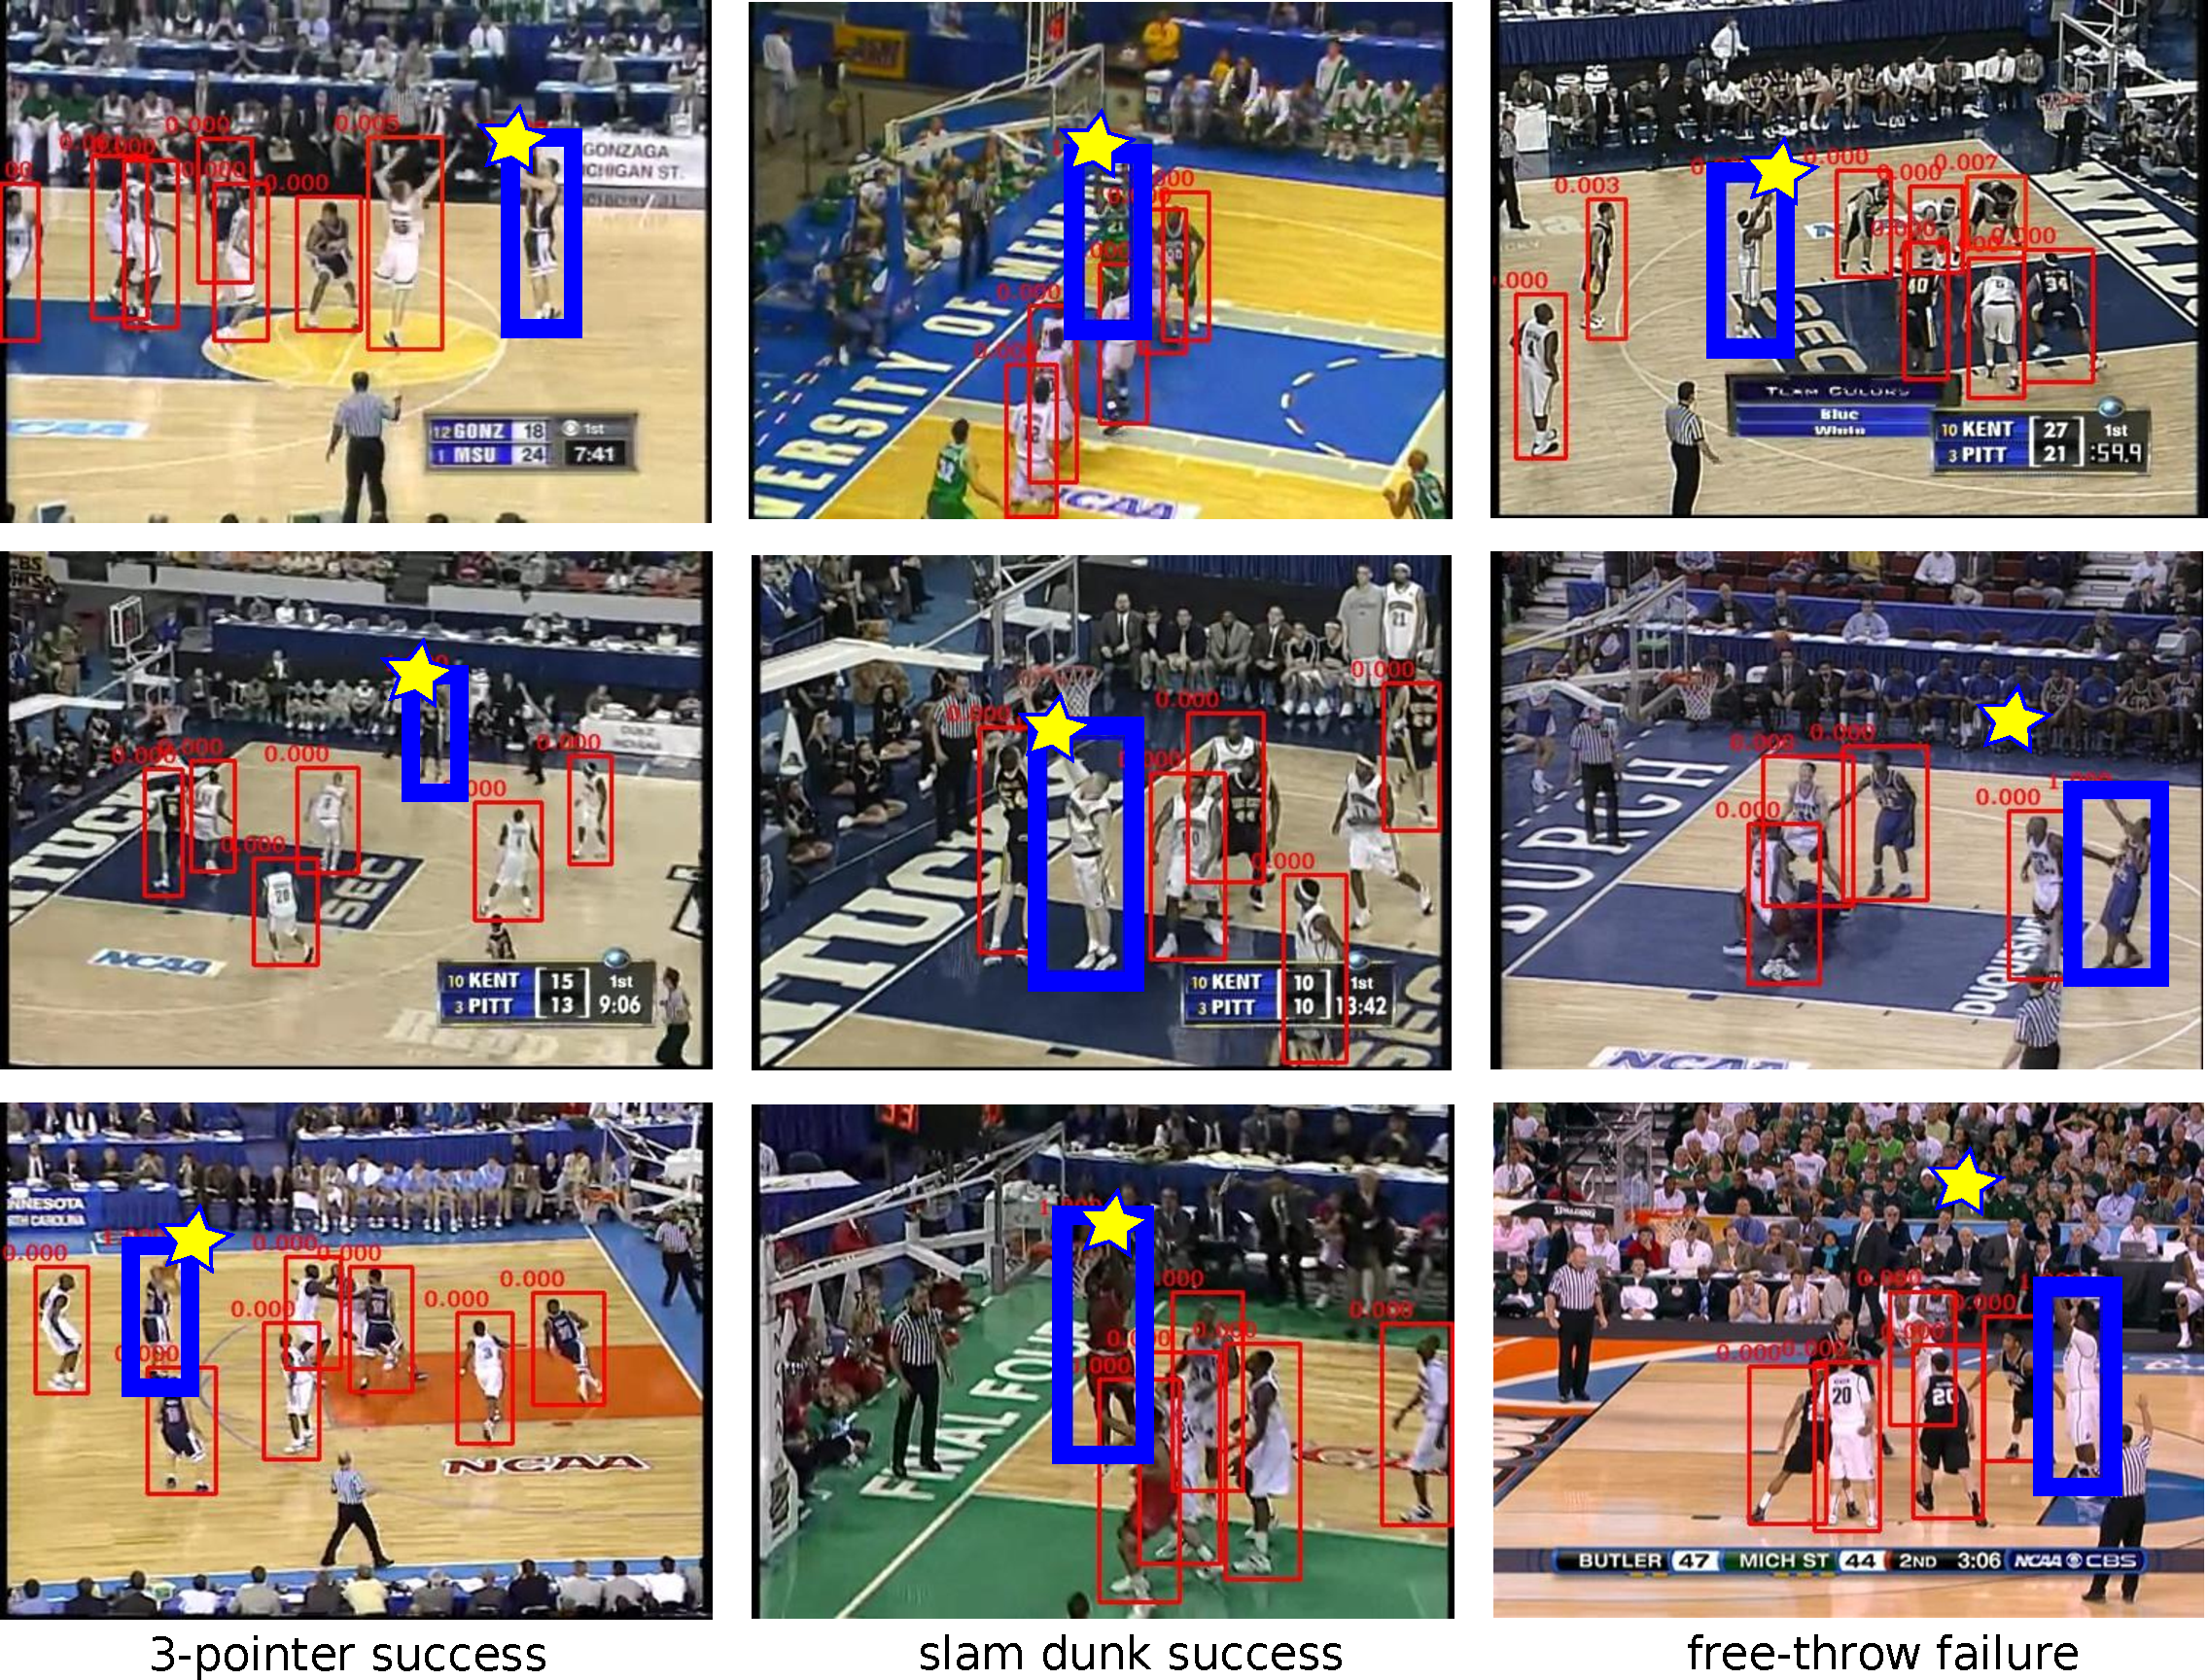
\includegraphics[width=1.0\linewidth]{images/visual_examples_v2.pdf}
\end{center}
   \caption{Visualization of our attention scores at the begining of different events
     for the tracking free model.
Each row of the event corresponds to a different video.
The player being attended is highglighted in blue.
The position of the ball is highlighted in yellow.}
\label{fig:visual_attention}
\end{figure*}
% ---------------------------------------------------------------------------------

% -------- Heat Map for youtube videos
\begin{figure}[t!]
\begin{center}
   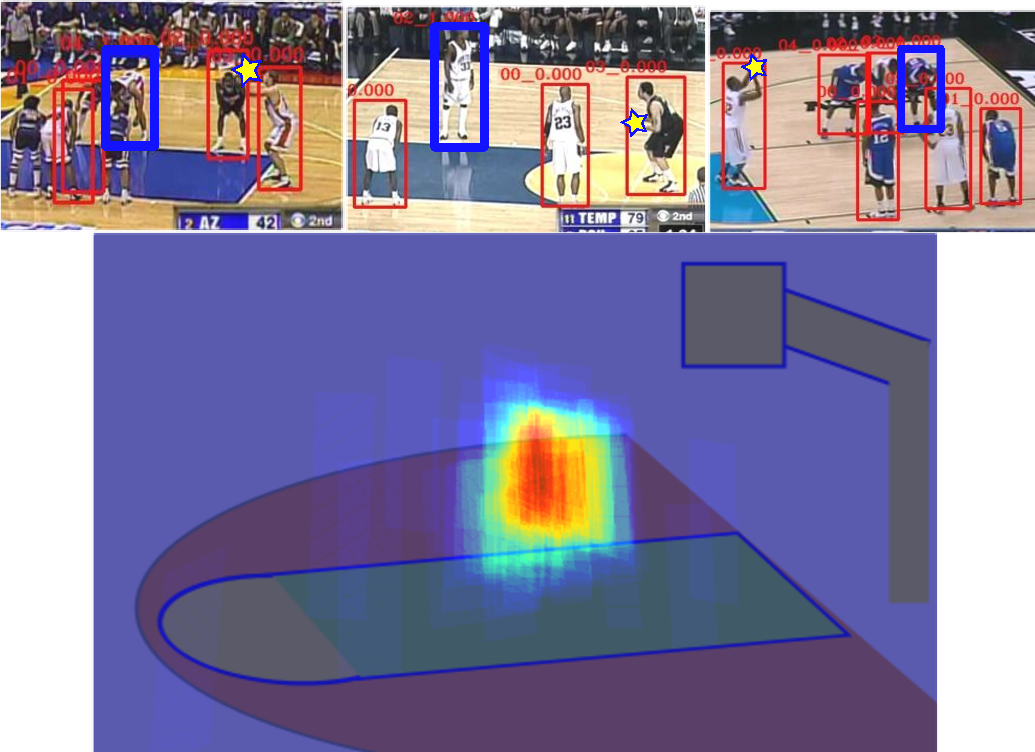
\includegraphics[width=1.0\linewidth]{images/track_spec_output.pdf}
\end{center}
   \caption{Visualization of attention scores at the begining of free-throw success
     for the attention model with tracks. In this setting, the model consistently
     attends to the defender at a particular spot.
   The player being attended is highglighted in blue, and ball is shown in yellow.}
\label{fig:visual_attention_trackspec}
\end{figure}
% ---------------------------------------------------------------------------------




\begin{table}[ht!]
\begin{center}
\small
 \begin{tabular}{|l|c|c|c|}
  \hline
Event            & Chance & Attn. with track & Attn. no track \\ \hline \hline
3-point succ.    & 0.333 & 0.445 & 0.519 \\ 
3-point fail.    & 0.334 & 0.391 & 0.545 \\ 
free-throw succ. & 0.376 & 0.416 & 0.772 \\ 
free-throw fail. & 0.346 & 0.387 & 0.685 \\  
layup succ.      & 0.386 & 0.605 & 0.627 \\ 
layup fail.      & 0.382 & 0.508 & 0.605 \\ 
2-point succ.    & 0.355 & 0.459 & 0.554 \\ 
2-point fail.    & 0.346 & 0.475 & 0.542 \\ 
slam dunk succ.  & 0.413 & 0.347 & 0.686 \\ 
slam dunk fail.  & 0.499 & 0.349 & 0.645 \\ \hline \hline  
Mean             & 0.377 & 0.438 & 0.618 \\ \hline
  \end{tabular}
\end{center}
  \caption{Mean average precision for attention evaluation.}
  \label{tab:attention_res}
\end{table}

To evaluate the attention models, we  labeled the player who was
closest (in image space) to the ball as the ``shooter''.
(The ball location is annotated in 850 test clips.)
We used these annotations to evaluate if our ``attention" scores
were capable of classifying the ``shooter" correctly in these frames.

The mean AP for this ``shooter"  classification is listed
in Tab.~\ref{tab:attention_res}.
The results show that the track-free attention model is quite consistent in picking
the shooter for several classes like ``free-throw succ./fail",
``layup succ./fail." and ``slam dunk succ.". This is a very
promising result which shows that attention on player detections
alone is capable of localizing the player making the shot. This could be
a useful cue for providing more detailed event descriptions
including the identity and position of the shooter as well.

Another interesting observation
%from Tab.~\ref{tab:attention_res}
is that the
attention scores for the tracking based model are less selective in focusing on
the shooter.  We observed that the tracking model is often reluctant to switch
attention between frames and tends to focus on a single player throughout the
event. This biases the model towards players who are present throughout the
event. For instance, in free-throws Fig.~\ref{fig:track_spec_att} we see that
the model always attends to the defender at a specific position, who is visible
throughout the entire event unlike the shooter.

In addition to the above quantitative evaluation, we wanted to
visualize the attention masks visually.
In order to make results comparable across frames, 
we annotated 5 points on the court and
aligned all the attended boxes for an event to one cannonical image. 
Fig.~\ref{fig:att_heatmap} shows a heatmap  showing the spatial distributions
of the attended players with respect to the court. It is interesting to note that
our model consistenly focuses under the basket for a layup, at the free-throw
line for free-throws and outside the 3-point ring for 3-pointers.

\eat{
Since basketball shots are often classified based on the position of the
shooter with respect to the court, we analyze this in
Fig.~\ref{fig:att_heatmap}.  We annotated specific points on the courts and
aligned all the attended boxes for an event to one cannonical image. We have
plotted the resulting heatmap showing the distribution in position of the
attended player with respect to the court. It is interesting to note that
our model consistenly focuses under the basket for a layup, at the free-throw
line for free-throws and outside the 3-point ring for 3-pointers.
}


% -------- Heat Map for youtube videos
\begin{figure*}[t!]
\begin{center}
%  \includegraphics[width=7 in]{images/attention_heatmap_full.pdf}
  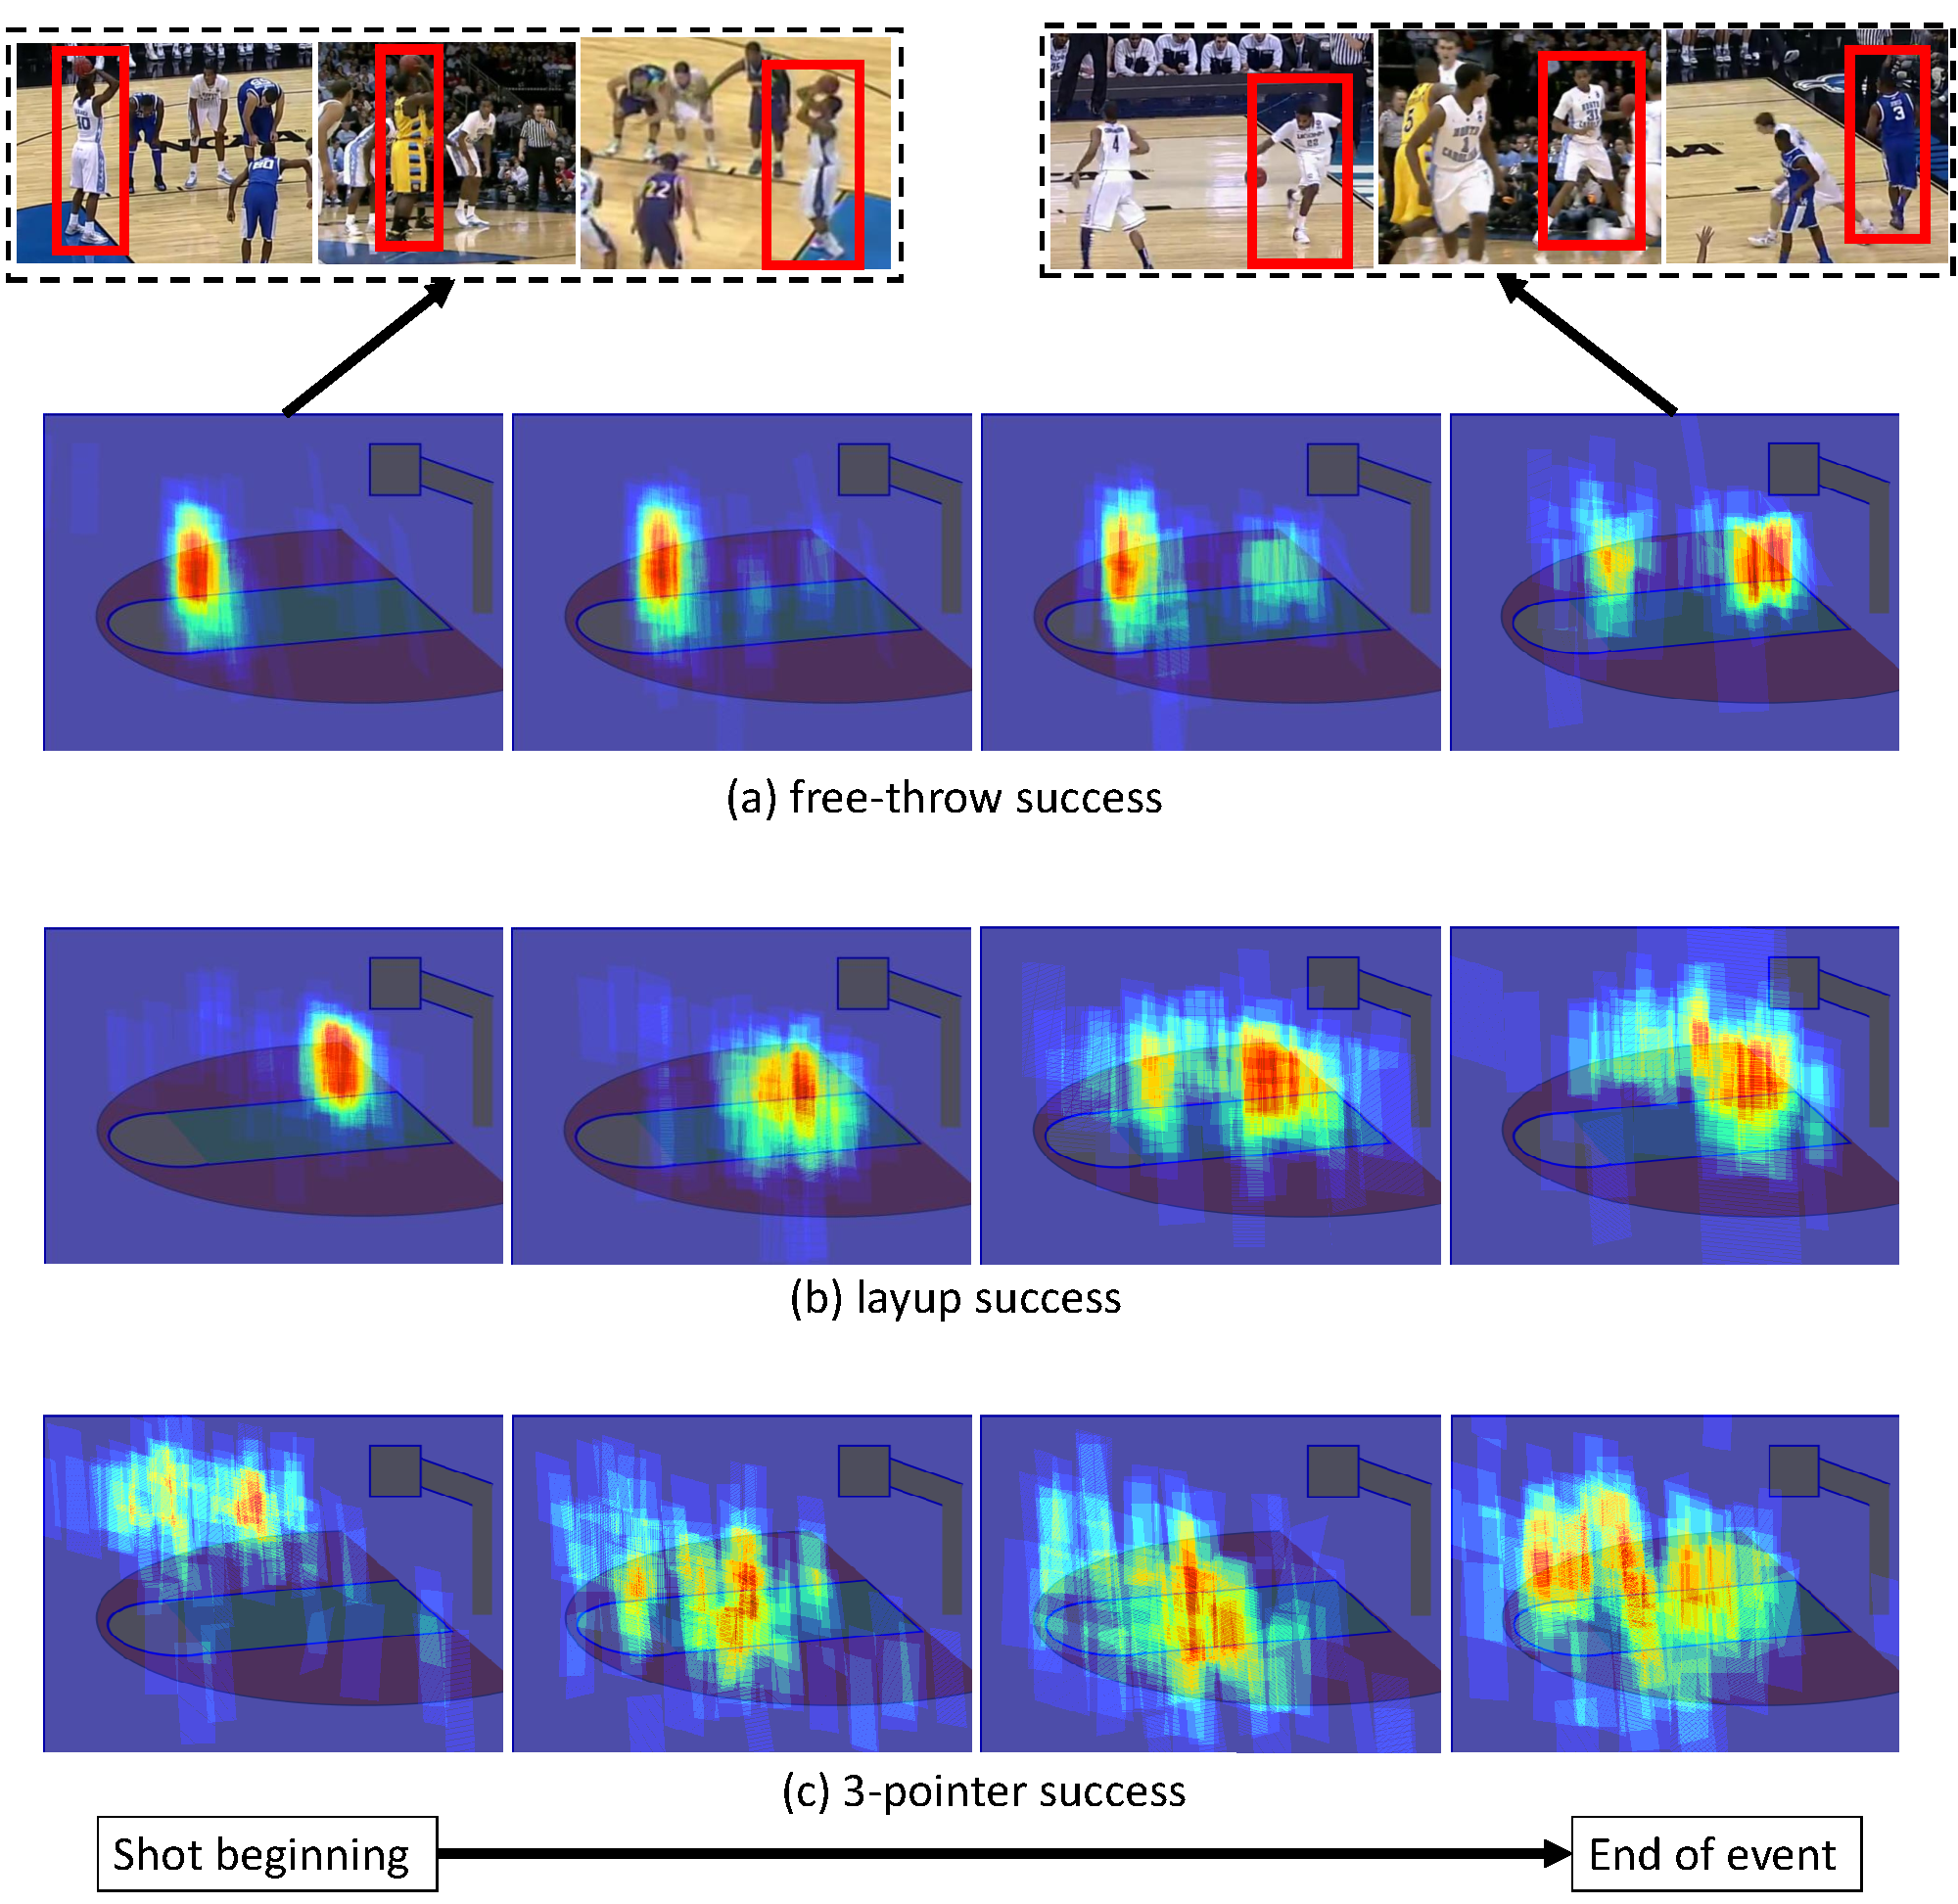
\includegraphics[width=7in]{images/heatmap_figure_cropped.pdf}
\end{center}
   \caption{We show the distribution of the attention over the basketball court
     for different events. We used an affine transform to transform the
     attended player's position to a cannonical frame for visualization.
     Interestingly, the attended court positions are the typical spots from
     which a player would make a shot for the corresponding event.
   }
\label{fig:att_heatmap}
\end{figure*}
% ---------------------------------------------------------------------------------


\section{Conclusion}
We have introduced a new attention based model for event classification and
detection in multi-person videos. Apart from recognizing the event, our model
can identify the key people responsible for the event without being explicitly
trained with such annotations. Our method can generalize to any
multi-person setting. However, for the purpose of this paper we introduced a
new dataset of basketball videos with dense event annotations and compared our
performance with state-of-the-art methods on this dataset.  We also evaluated
the ability of our model to recognize the ``shooter" in each of the events with
visualizations of the spatial locations attended by our model.  A simple
extension to our model would be the use of dense-flow features in addition to
appearance features, and could lead to a performance gain.


{\small
\bibliographystyle{ieee}
\bibliography{bballbib}
}

\end{document}
